%%「論文」,「レター」,「レター(C分冊)」,「技術研究報告」などのテンプレート
%% v3.2 [2019/03/19]
\documentclass[technicalreport]{ieicej}

%% 4. 「技術研究報告」
%\usepackage[dvips]{graphicx}
\usepackage[dvipdfmx]{graphicx,xcolor}
\usepackage[T1]{fontenc}
\usepackage{lmodern}
\usepackage{textcomp}
\usepackage{latexsym}
\usepackage[fleqn]{amsmath}
\usepackage{amssymb}

\jtitle{音響信号の非現実的ミックスの検出}
\jsubtitle{}
\etitle{Study on detection of mixing unreality for PCM audio signal}
\esubtitle{}
\authorlist{%
 \authorentry[sonoda@cis.nagasaki-u.ac.jp]{薗田 光太郎}{Kotaro SONODA}{NU}
% \authorentry[メールアドレス]{和文著者名}{英文著者名}{所属ラベル}
}
\affiliate[NU]{長崎大学~大学院~工学研究科\\〒852--8521 長崎県長崎市文教町1--14}{Graduate School of Engineering, Nagasaki University\\Bunkyo-machi 1--14, Nagasaki, Nagasaki 852-8521, Japan}
%\affiliate[所属ラベル]{和文勤務先\\ 連絡先住所}{英文勤務先\\ 英文連絡先住所}

\begin{document}
\begin{jabstract}
%和文あらまし
近年,音の模擬合成手法の発展により,人工的な模擬合成音は,現実の録音そのものであると聴覚的に認識されてもおかしくないほどとなりつつある.しかし,聴覚的には自然に感覚されても,現実の録音ではあり得ない波形に合成される場合もある.楽曲制作で一般的に用いられるマルチトラックレコーディングとミキシング過程では,異なる環境で収録された複数の音源を別の統一された環境下に配置合成される.既報では音源の再配置における位相パンニング処理の有無の検出手法について検討をおこない,左右チャネル間群遅延差の標準偏差が極端に低い場合に位相パンニング処理があったことを疑われることを示した.今回の報告ではマルチトラックミキシングを考慮した手法を検討する.
\end{jabstract}
\begin{jkeyword}
%和文キーワード
\end{jkeyword}
\begin{eabstract}
%英文アブストラクト
\end{eabstract}
\begin{ekeyword}
%英文キーワード
\end{ekeyword}
\maketitle

\section{はじめに}
現代の音楽制作現場では,計算機の利用により簡単にデジタル音響加工を行うことが可能となった.商用の楽曲メディアでは,現実に直接録音された音に対して,残響処理や各種エフェクトを施し,さらにそれらを適切な時刻,到来方向に配置するなどを行うのが一般的になっている.また,深層学習の導入により,簡単に人間には現実の音と聞き分けることができない高品質な模擬音を作成し,音源とすることも可能である.このような音源・音場の模擬は,人間による聴取においては問題にならないが,真正性の担保が必要とされるシステムにおいては大きな問題となる可能性がある.一旦パッケージ化された信号についてその真正性を担保するには,真正の配信者が介在し,恣意的に電子透かしを埋め込んだり,フィンガープリントを記憶するなどによりそれらを照合することで解決できるが,パッケージされる前の直接録音されたものである真正性を担保することにはならない.事実,音声による個人認証・照合システム(ASV: Automatic speaker verification)では,このような録音再生音(リプレイ音声)やディープフェイク音声などによる詐称がシステムの判断を誤らせる障害となることが取りざたされている, 
音声以外でも例えば,工場の異常音を模擬した音が作成され,再生された場合,労働者に誤った判断をさせてしまう.

\begin{figure}[tbh]
	\centering
	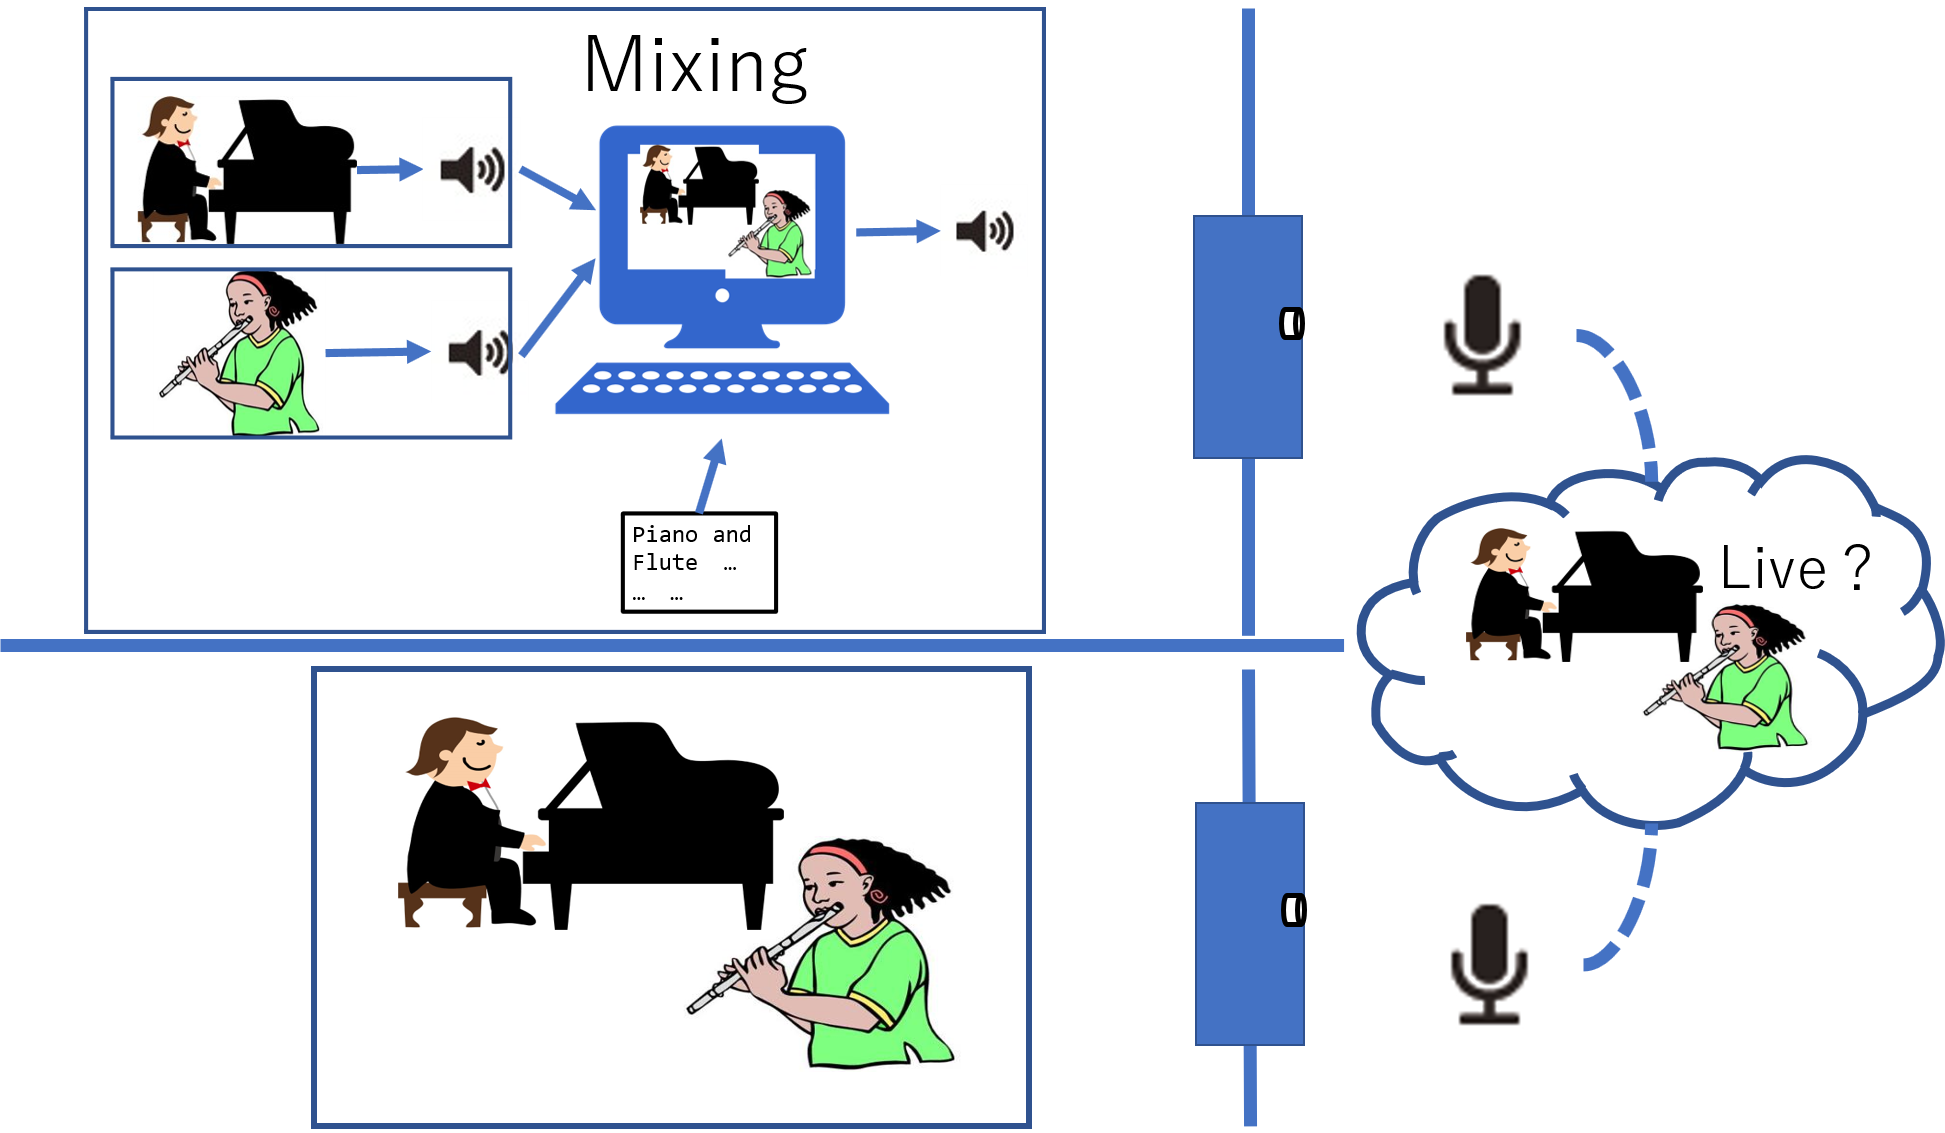
\includegraphics[width=0.5\textwidth]{fig/Anti-spoofing.png}
	\caption{Anti-spoofing: 手元の録音はライブ音かなりすまし加工音か.}
	\label{fig:Anti-Spoofing}
\end{figure}
%図が必要か
%        発生音(A)  録音(B)    加工音/模擬音源/パッケージ化された音(C) 通信データ    受信した音(D)
% 音の発生 -->録音---------->加工--------->(パッケージ化)--------------->送信(再生)-------->受信-------->
%                          
% 改ざん検知(電子透かし埋込やフィンガープリント記憶):C-D間
% なりすまし検知:B-D間


このような直接録音・現実音場の模擬加工の検知(Anti-spoofingは,音声その他のバイオメトリクス認証においては生体検知(Liveness detection / PAD: presentation attack detection\cite{ISO/IEC30107-1:2016})として考えられ,ASV-PADについてはその検知性能を競うASVspoof challenge\cite{ASVspoof,ASVspoof2015,ASVspoof2017}が開催されている. 

\section{チャネル間群遅延差によるパンニング加工の検出.モノラル音の擬似ステレオ化}
本章では,既報\cite{kuroda_EMM201903}のIGDD (チャネル間群遅延差; Inter-channel Group-Delay Difference)について概要を述べる.
いま,検出対象とする信号は2chステレオ信号とする.この信号が,実在する音源に対してその場で録音された信号(ライブ信号)なのか,ある1チャネル音源信号をステレオパンニングで擬似ステレオ化された信号(加工信号)なのかを検出したい.既報では,加工信号ではチャネル間の群遅延差 Inter-channel Group-Delay Difference (以下IGDD) すなわち到来角度差が信号全体の中で変化しにくいと考えられることに着目した.対してライブ信号では,各チャネルの信号が録音時の音源ー各センサ間で決定され,チャネル間の到来角度差は加工音に比べ変化しやすいと考えられる.この考えに基づき,以下の式\eqref{IGDD}の指標をライブネス度(ライブ信号らしさ)とした.
\begin{equation}
	\mbox{liveness}_{\mbox{IGDD}} = \mbox{stdv}_n\left[ \mbox{ave}_k[ \mbox{IGDD}(k,n)] \right] \label{IGDD}
\end{equation}

新たにスタジオ録音したライブ信号(A),それをステレオパンニングした加工信号(B),パッケージ化されたクラシック音楽信号(ワントラックと想定)(C),ポップス音楽信号(マルチトラックと想定)(D)について評価した結果,加工信号である(B)(D)の評価値は,ライブ信号である(A)(C)に比べ大幅に低い値をとることが確認された.

音声の生体検知性能を競うASVSpoofにおける生体発話/スピーカ再生の識別においては,検出対象を2chステレオ信号した場合に,マイク間(チャネル間)の到来時間差に基づく手法が多く提案されている.実発話の場合は,発話位置が口内で前後するため,左右チャネルへの到来時間の差が変化しやすく,対してスピーカ再生の場合には発音位置が変化しないためチャネル間の信号の差は時間差が優位をしめる.したがって,スピーカ再生のに対する録音信号で,チャネル間到来時間差を求める指標であるチャネル間GCC(Generalized Cross-Correlation)\cite{GCC}が高くなりやすいことを利用している.式\eqref{eq:GCC}に時間系列$x(t)$と$y(t+\tau)$の$GCC(\tau)$を示す.

\begin{equation}
GCC(\tau) = \mathcal{F}^{-1}\left[X(\omega)Y(\omega)^{*}{\rm e}^{j\tau\omega}\Phi(\omega)\right] \label{eq:GCC}
\end{equation}
ここで,$X(\omega)$および$Y(\omega)$は$x(t)$および$y(t)$のFourier変換であり,$\Phi(\omega)$は前2項で構成されるクロススペクトルに対する一般化周波数フィルタである.$\Phi(\omega)$をクロススペクトル絶対振幅値とすれば式\eqref{eq:GCC}は白色化クロススペクトルの逆Fourier変換と考えられる(GCC-PHAT;GCC-PHAse Transform).

さらに矢野・塩田らは,音声の生体検知でありながら,発話中に現れる無声区間の背景音のGCCに着目し,背景音においても,実録音(ライブ録音)に比べ大幅にスピーカ再生音のGCCが高くなることを利用し,識別性能を向上させている\cite{groundICGCC}.
GCCは仮定する到来時間差$\tau$としたときの相関係数であり,我々のチャネル間群遅延差の散らばりが少ないことと同様の考え方に基づく.

しかし,これらの手法は,エコー・リバーブ環境下では真の到来時間差・群遅延差を計測できず,評価値の性能が悪い.

\section{マルチトラックミキシングの検出}

ASVspoofで対象としているスピーカ再生音声は,実発話録音音声のスピーカ再生を再録音したものであり.再録音された信号は再生信号(実発話録音)と再生再録音時の背景音との合成および,再生再録音時の室内伝達関数との畳み込みと考えられる.元の再生信号じたいも実発話録音時の室内伝達関数との畳み込みであるため,1個の信号全体の中で,録音環境(室内伝達関数)が変化することとなる.矢野・塩田らの無声区間GCCに着目した手法は,無声区間では実発話録音時の環境が現れず,スピーカ再生環境のみとなるため性能向上したと考えられる.

一般の音響信号の場合,ライブ信号は,多数の方向から到来する実発音を一挙録音したものとする,一方で加工音は個々の楽器音の録音(マルチトラック)を加工合成(ミキシング)したものとする.ライブ信号がある特定の環境で一貫して録音されたものであるのに対し,加工音は録音環境の異なる音源が加算・時刻配置されたものである.

そこで,チャネル間ではなく,隣接する時間フレーム間での録音環境の急激な変化をとらえることとする.前節の到来方向も録音環境と考えることができるが,マルチトラックミキシングを捉えることはできない.ここでは,残響特性に着目することとする.

残響特性は,音源に対するフィルタ(畳み込み処理)であり,観測信号のケプストラム上では加算の関係になる.観測した信号を$y(t)$とすると,$y(t)$は式\eqref{tconv}のように音源信号$s(t)$と残響特性を$h(t)$の畳み込み演算(積和演算)でモデル化でき,Fourier変換ドメインのスペクトルでは,式\eqref{spectrum}のようにアダマール積となる.この両辺に対して対数をとったものは加算の関係となり,そのFourier変換(すなわちケプストラム)でも式\eqref{cepstrum}のように加算となる.
\begin{gather}
y(t) = s(t) * h(t) \label{tconv}\\
Y(\omega) = S(\omega) \cdot H(\omega) \label{spectrum}\\
\mathcal{Y}(q) = \mathcal{S}(q) + \mathcal{H}(q) \label{cepstrum}
\end{gather}
ここで$Y(\omega), S(\omega), H(\omega)$は角周波数$\omega$におけるスペクトル,$\mathcal{Y}(q), \mathcal{S}(q), \mathcal{H}(q)$はquefrency:$q$におけるケプストルとする.

音源信号は逐時変化するが,残響特性は環境が変化しない限り大きくは変化しない\cite{yYyOyY_ExtRTFbHSP_MASJ2014s}と考えられるので,仮に実録音時の残響特性のケプストラム$\mathcal{H}_{\o}(q)$を得ることができれば,観測信号のケプストラム$\mathcal{Y}_{n}(q)$とのケフレンシードメインの相互相関$\mathcal{C}_{\o}(\tau)$は,観測時の残響特性のケプストラム$\mathcal{H}(q)$との相互相関を強く反映したものとなることが予想される.ただし,相互相関を求めるために,ケプストラムは位相特性を考慮しない振幅ケプストラムの実部とする.

フレーム$n$のケプストラムを$\mathcal{Y}_{n}(q)$とすると,このフレームに関する正規化相互相関係数$\mathcal{C}_{\o}(n)$は式\eqref{CrossCepstrum}で求められる.
\begin{gather}
\mathcal{C}_{\o}(n) 
= \frac{%
	\sum_{q}\mathcal{Y}_{n}(q)\mathcal{H}_{\o}(q)
}{%
\sqrt{\sum_{q}\mathcal{Y}_{n}(q)^2\sum_{q}\mathcal{H}_{\o}(q)^2}
} \label{CrossCepstrum}
\end{gather}

実録音を示す参照信号$\mathcal{H}_0$は,信号中で最もパワーの低いフレーム(無音区間)で得られる短ケフレンシーケプストラムを採用する.

$\mathcal{C}_{\o}(n)$がある閾値$\mathcal{c}_{\o}$を下回るとき,フレーム$n$は,実録音とは異なる環境のトラックがミックスされたことを意味すると考える.

\section{評価実験}

評価音源として,新たにスタジオ録音したギター演奏\#live,騒音データベース\ref{Souon}から\#env,時間方向に\#liveと\#envを連結した\#concat, \#envの音源の途中に\#liveを加算した\#mix, RWC研究者用音楽データベース\ref{RWC}からポピュラー音楽\#pops,ジャズ音楽\#jazz,を用意した.いずれも1チャネル音源とし,フレーム内で量子化振幅値がすべて0となる区間は現れないものとする.

\#live および \#env は加工されていない信号(ライブ信号)と考える.\#concatおよび\#mixは環境の異なるライブ信号を合成したものである.\#popsはマルチトラックミキシングが行われており,\#jazzは明記されていないが一般に一挙録音されたものと考える.

\begin{figure}
	\centering
	\includegraphics[width=\textwidth]{#live.pdf}
	\caption{#live}
	\label{fig:result_live}
\end{figure}
\begin{figure}
	\centering
	\includegraphics[width=\textwidth]{#env.pdf}
	\caption{#enc}
	\label{fig:result_env}
\end{figure}
\begin{figure}
	\centering
	\includegraphics[width=\textwidth]{#concat.pdf}
	\caption{#concat}
	\label{fig:result_concat}
\end{figure}
\begin{figure}
	\centering
	\includegraphics[width=\textwidth]{#mix.pdf}
	\caption{#mix}
	\label{fig:result_mix}
\end{figure}
\begin{figure}
	\centering
	\includegraphics[width=\textwidth]{#pops.pdf}
	\caption{#pops}
	\label{fig:result_pops}
\end{figure}
\begin{figure}
	\centering
	\includegraphics[width=\textwidth]{#jazz.pdf}
	\caption{#jazz}
	\label{fig:result_jazz}
\end{figure}

\figref{fig:result_live}から\figref{fig:result_jazz}に各信号の信号波形と対応する時刻のケプストラム相互相関計数の変化を示す.信号の合成のない\#live(\figref{fig:result_live}),\#env(\figref{fig:result_env})ではある一定の範囲内で変動しているが,ミキシングのあった\#concat(\figref{fig:result_concat})および\#mix(\figref{fig:result_mix})では連結されたフレームや合成がなされたフレームで大幅に値が変化していることが見てとれる.




\section{結論}
本報告では,短ケフレンシー領域のケプストラムを録音環境と考え,信号中で最もパワーの低いフレームで得られる短ケフレンシーケプストラムを実録音環境とした上で,信号中の各フレームでの相互相関係数の変化を計測し,急峻に低下するフレームを非現実的ミックスフレームとした.


\bibliographystyle{sieicej}
\bibliography{emm202001}

\end{document}